\section{Introduction}
WASM (or WebAssembly), is an open standard binary code format close to assembly. It is independent of the platform and can be compiled from other languages. WASM is an open standard whose initial objective is to offer a competitive performance compare with native code and same compatibility with the current web ecosystems. However, due to its appealing property of portability, security and speed, its usage start to arise in distributed cloud and edge computing. Recently it becomes a popular binary format for users to running customized functions on AWS Lambda, Open Yurt, AZURE, etc.

As with the technology of WASM run-time for edge-computing shifts, security and privacy issues emerge. For instance, in the cloud or edge computing scenario, we need to trust that the calculation is performed as defined so that the result is trustworthy. In the private computing scenario, a user needs to prove to another entity that it possesses certain private information without revealing it.

ZKSNARK recently proves to be a desired technique to resolve the trustless and privacy demand for trustless distributed computing. However, adoption of ZKSNARK usually requires the program being written in arithment circuits (see Section \ref{chp:arith-circuits}). This barrier make it hard to apply ZKSNARK on existing programs. Thus in this paper, we propose a novel way to apply ZKSNARK to existing WASM applications running on trustless computing entities by implementing \zkwasm, a ZKSNARK backed WebAssembly virtual machine. By using \zkwasm, the computation provider can prove to any user that the computation result is computed honestly from the confirmed code and no privacy information is leaked.

\subsection{Succinct Verification}
Succinct non-interactive arguments (SNARGs) enable verifying NP statements with lower complexity than required for classical NP verification. Traditionally, the focus has been on minimizing the length of such arguments; nowadays researches have focused also on minimizing verification time, by drawing motivation from the problem of delegating computation.

Recent constructions of preprocessing SNARGs have achieved attractive features: they are publicly-verifiable, proofs consist of only O(1) encrypted (or encoded) field elements, and verification is via arithmetic circuits of size linear in the NP statement. Additionally, these constructions seem to have “escaped the hegemony” of probabilistically-checkable proofs (PCPs) as a basic building block of succinct arguments.


\subsection{Polynomial Commitment Schemes}
PCS (Polynomial Commitment Schemes \cite{boneh2020halo-pcs,boneh2020efficient-pcs,kate2010polynomial-pcs}) is a powerful tool to construct SNARK schemes for the statement of polynomial evaluation. PCS provides a way for prover and verifier to commit to a polynomial $p$ and then open the commitment at certain any point (prove that the evaluation of $P$ a point $x$ is equal to a claimed value $v$). In this paper, if without specification, We use KZG (Kate, Zaverucha and Goldberg) as our polynomial commitment scheme. KZG protocol contains four parts: 
\begin{itemize}
\item $(vk,pk)\leftarrow\texttt{setup}(\tau, 1^\lambda):$ For some security parameter $\lambda$, sample randomly $\tau \leftarrow \mathbb{F}_r$ and then compute $pk=\tau^i\mathbb{G}_1$ for $i\in\{1,\dots,m\}$ and $vk=\tau \mathbb{G}_2$.
\item $C\leftarrow\texttt{commit}(pk,p):$ given the polynomial $p(x)\in \mathbb{F}_r[x]$ and the proving key $pk$, compute $C=p(\tau)\cdot\mathbb{G}_1=\sum_{i=0}^{n<m}p_i\cdot\tau^i\mathbb{G}_1$ 
\item $\pi\leftarrow\texttt{open}(p, y, z):$ to prove that $p(z)=y$, compute the polynomial $q(x)=(p(x)-y)/(x-z)$ and then the proof $\pi=q(\tau)\cdot\mathbb{G}_1$
\item $\texttt{bool}\leftarrow\texttt{verify}(C, \pi, vk):$ compute $P_z=z\mathbb{G}_2$ and $P_y=y\mathbb{G}_1$, and then verify that $e(\pi, vk-P_z)=e(C-P_y,\mathbb{G}_2)$
\end{itemize}
\subsection{Stateless Programs as Arithmetic Circuits}
\label{chp:arith-circuits}
Once there exists a SNARK scheme for a prover to prove the evaluation of polynomials $p_i$ at $x_i$ to a verifier, we can then construct SNARK for a prover to prove that a program $P(X)$ has certain return value $v$ when input $X$ is provided. Many such construction can be found in literature such as Groth, Sonic, Marlin, Plonk, etc. In this paper, we construct our ZK virtual machine using the proof system of Halo2, which is an extension of PLONK (See Section \ref{chp:constraint-system}). In PLONK setup, stateless programs can be encoded into a special format called arithmetic circuits.

An arithmetic circuit is a set of gates and each gates can have a set of inputs that need to be processed and a set of outputs that can be used as other gates' inputs. The gates can be connected together so as to carry out an arithmetic algorithm. In the end, the outputs of the circuit is result of the algorithm. For example, suppose that we need to represent an sum algorithm can be constructed by a list of add gates as in Figure \ref{fig:sum-gates}.

\begin{figure}[!ht]
\centerline{
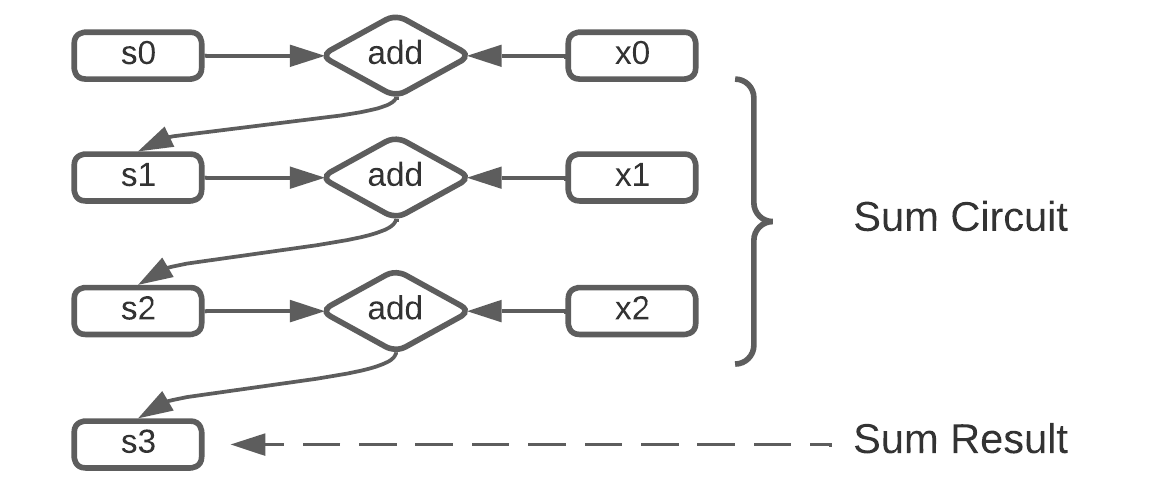
\includegraphics[scale=0.8]{figs/arithment-circuit.png}
}
\caption{Arithment Circuit of Sum}\label{fig:sum-gates}
\end{figure}

Now we have connected stateless programs to arithmetic circuits, and we know how to construct SNARKS of polynomial evaluation using PCS. Therefore it remains to establish a connection between arithmetic circuits with polynomials. This can be achieved by using interpolation techniques and copy constraints in PLONKish (see Section \ref{chp:constraint-system}).

%PCS 是polynomialbase的,constraint base ---> PCS
\subsection{Encoding Stateful Virtual Machine in Arithmetic Circuits}
Now we need to make a setup further, instead of construct a SNARK sheme for Stateless programs, we would like to construct a SNARK scheme for a stateful virtual machine. We do not constructing such SNARK from scratch, we construct it from the knowing ingredients which are the SNARK of programs execution and evaluation of polynomials. 

To start with, we establish the connection between a virtual machine and a program by treating the virtual machine as a composition of state transition and each transition is defined as a monad function between states. We denote the transition function as $T$ which takes two inputs $o:Opcode$ and $s:State$
and the output of $T$ is a new state $s':S$. The type of state $\mathcal{S}$ is defined as a tuple of \fullstate \, where $\mathcal{F}$ is the calling frame, $\mathcal{M}$ is the memory state, $\mathcal{S}_p$ is stack and $\mathcal{I}$ is the image which contains code image $\mathcal{C}$ and initial memory $\mathcal{H}$.

With this setup we can mapping execution of a executable image $I$ in a virtual machine $\mathcal{V}_m$ as a sequence of transition function $t_i \in T$ over an initial state $s_0 \in \mathcal{S}$. Also we denote $s_i = t_i (o_i, t_{i-1}(o_{i-1}, \cdots t_0(o_0, s_0)))$ and $s_e$ to be the last state of the transition sequence.

In the end, make sure that the last state $s_e$ is indeed our desired state, we need to enforce two more things. First, the final opcode $o_{e-1}$ is return and the depth of the calling frame of $s_e$ is zero $\mathcal{F}(s_e).depth = 0$. Second, semantic of each transition $t_i$ defined by opcode $o_i$ is enforced.

%Stateless -> Statefull 的虚拟机:monadic function while s is hash
\subsection{Leverage zero-knowledge in ZKWASM}
A zk-SNARK is a SNARK scheme that provide a way for a prover to prove statements without leaking any information. When we construct the above SNARK scheme for virtual machine in a zero-knowledge way, then we create a ZK Virtual machine that can prove the execution of certain program image without leaking any information.  This feature makes the ZK virtual machine extremely useful in scenarios where the prover would like to prove that certain ouput is calculated from execution a particular program image but does not want to leak the data used.
 
\subsection{Our contribution}
In this paper we proposed and implemented the first zk-WASM virtual machine that supports web assembly specification.
